\documentclass[12pt]{article}
\usepackage{latexsym}
\usepackage{graphicx}
\title{Problem Set 6}
\author{Shun Zhang (sz4554)}

\begin{document}

\maketitle

\textbf{Part A}

\textbf{8.4.1}

\begin{tabular}{l|l l l l}
	Action & No Index & Star Index & Moview Index & Both Indexes\\
	\hline
	$Q_1$ & 100 & 4 & 100 & 4\\
	$Q_2$ & 100 & 100 & 4 &  4\\
	I & 2 & 4 & 4 & 6\\
	\hline
	Average & $2+98p_1+98p_2$ & $4+96p_2$ & $4+96p_1$ & $6-2p_1-2p_2$ \\
\end{tabular}
\\

\textbf{14.2.1}

a)

i) We need $1000000/10=100000$ blocks for storing data. For these data, we need $1000000/(70-1)=14493$ leaf nodes. Assume leaves are on the d-th layer. (d-1)th layer has $14493/70=208$ nodes. (d-2)th layer has $208/70=3$ nodes. (d-3)th layer should be the root. It has one node has 3 pointers. The total number of blocks are $100000+14493+208+3+1=114705$.

ii) The B-tree has 4 layers. There is another retrieval for data block. 5 times in total.

b)

Same results as (a). Make sure that pointers on the leaves point to the right block - even though data are not in order.

c)

i) We need $1000000/10=100000$ blocks for storing data. For these data, we need $100000/(70-1)=1450$ leaf nodes. Assume leaves are on the d-th layer. (d-1)th layer has $1450/70=21$ nodes. (d-2)th layer should be the root. It has one node has 21 pointers. The total number of blocks are $100000+1450+21+1=101472$.

ii) The B-tree has 3 layers. There is another retrieval for data block. 4 times in total.
\\

\textbf{14.2.2}

a)

i) The blocks are exactly the same.

ii) We start from the lower bound, visit along the leaves layer. It visits 3 interior nodes, $1000/69=15$ leaves, $1000/10=100$ data blocks. $3+15+100=118$ retrievals in sum.

b)

i) The blocks are exactly the same.

ii) We start from the lower bound, visit along the leaves layer. It visits 3 interior nodes, $1000/69=15$ leaves, 1000 data blocks (they are not guaranteed to be in the same block). $3+15+1000=1018$ retrievals in sum.

c)

i) The blocks are exactly the same.

ii) We start from the lower bound, visit along the leaves layer. It visits 2 interior nodes, $1000/10/69=2$ leaves, $1000/10=100$ data blocks. $2+2+100=104$ retrievals in sum.
\\

\textbf{Part B}

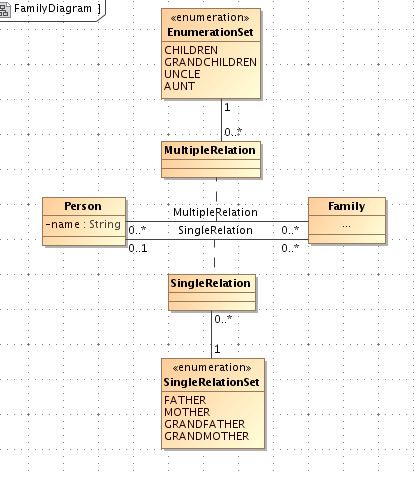
\includegraphics[width=80mm]{family.png}

\end{document}
